% Contributions are much appreciated, in order to contribute to this project, head over to this repository:
% https://github.com/bshramin/uofa-eng-assignment

\documentclass[11pt,letterpaper]{article}
\textwidth 6.5in
\textheight 9.in
\oddsidemargin 0in
\headheight 0in
\usepackage{graphicx}
\usepackage{fancybox}
\usepackage[utf8]{inputenc}
\usepackage{epsfig,graphicx}
\usepackage{multicol,pst-plot}
\usepackage{pstricks}
\usepackage{amsmath}
\usepackage{amsfonts}
\usepackage{amssymb}
\usepackage{eucal}
\usepackage[left=2cm,right=2cm,top=2cm,bottom=2cm]{geometry}
\usepackage{esvect}
\pagestyle{empty}
\DeclareMathOperator{\tr}{Tr}
\newcommand*{\op}[1]{\check{\mathbf#1}}
\newcommand{\bra}[1]{\langle #1 |}
\newcommand{\ket}[1]{| #1 \rangle}
\newcommand{\braket}[2]{\langle #1 | #2 \rangle}
\newcommand{\mean}[1]{\langle #1 \rangle}
\newcommand{\opvec}[1]{\check{\vec #1}}
\renewcommand{\sp}[1]{$${\begin{split}#1\end{split}}$$}

\usepackage{lipsum}

\usepackage{listings}
\usepackage{color}
\usepackage{wrapfig}
\usepackage[shortlabels]{enumitem}

\definecolor{codegreen}{rgb}{0,0.6,0}
\definecolor{codegray}{rgb}{0.5,0.5,0.5}
\definecolor{codepurple}{rgb}{0.58,0,0.82}
\definecolor{backcolour}{rgb}{0.95,0.95,0.92}

\lstdefinestyle{mystyle}{
	backgroundcolor=\color{backcolour},   
	commentstyle=\color{codegreen},
	keywordstyle=\color{magenta},
	numberstyle=\tiny\color{codegray},
	stringstyle=\color{codepurple},
	basicstyle=\footnotesize,
	breakatwhitespace=false,         
	breaklines=true,                 
	captionpos=b,                    
	keepspaces=true,                 
	numbers=left,                    
	numbersep=5pt,                  
	showspaces=false,                
	showstringspaces=false,
	showtabs=false,                  
	tabsize=2
}

\lstset{style=mystyle}

\begin{document}
\pagestyle{plain}

\begin{flushleft}
Estudiante: Fabio Quimbay\\
Email: fabio.quimbay883@comunidadunir.net\\
Profesor: Miguel Ángel Cabeza\\
Fecha: Noviembre 9 de 2022\\
\end{flushleft}

\begin{flushright}\vspace{-20mm}

\includegraphics[height=2cm]{logo.png}
\end{flushright}
 
\begin{center}\vspace{0cm}
\textbf{\large PER5786 2022-2023  Física 1 (GFI) - PER5786 2022-2023}\\
 Tema 3 - Movimientos elementales
\end{center}

 
\rule{\linewidth}{0.1mm}
%%%%%%%%%%%%%%%%%%%%%%%%%%%%%%%%%%%%%%%%%%%%%%%%%%%%%%%%%%%%%%%%%%%%%%%%

\bigskip
\bigskip

%%%%%%%%%%%%%%%%%%%%
\textbf{Problema propuesto 1}\\

\begin{wrapfigure}{r}{0.25\textwidth}
\begin{center}
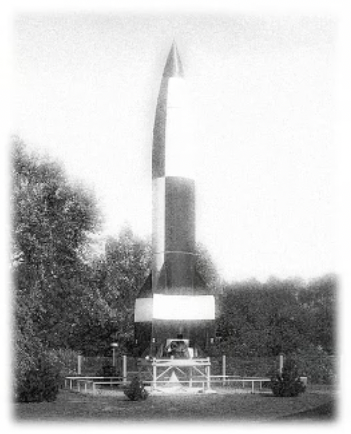
\includegraphics[width=0.25\textwidth]{problema_1.png}
\end{center}
\end{wrapfigure}

Durante unas pruebas de vuelo vertical realizadas el 3 de octubre de 1942, el cohete alemán 18014 de la empresa Mittelwerk GmbH fue el primer objeto en superar la "línea Kármán" (a 100 km. de altura) que define la separación entre espacio y atmósfera a efectos astronáuticos internacionales. Sabiendo que dicho cohete alcanzó una altura de 189 km, calcula con qué velocidad terminó por impactar en la tierra. Desprecia el rozamiento atmosférico, y aproxima $g=9.8\,m/s^2$.\\

\textbf{Formulas base:}\\

Se tomarán las siguientes formulas base del MRUA:

\begin{align}
\boxed{ V = V_{0} + a \cdot (t - t_{0})^2}\\
\boxed{ e = e_{0} + V_{0} \cdot (t - t_{0}) + \frac{1}{2} \cdot a \cdot (t - t_{0})^2 }
\end{align}

\textbf{Solución:}\\

Es necesario organizar los parámetros dados, a saber:

\begin{align*}
e &= 189\,k = 189000\,m\\
e_{0} &= V_{0} = t_{0} = 0\\
g &= -9.8\,m/s^2
\end{align*}

De tal manera, se pueden reorganizar las ecuaciones de la siguiente forma, a saber:

\begin{align}
\boxed{ e = \frac{1}{2} \cdot a \cdot t^2 }\\
\boxed{ V_{y} = a \cdot t}	
\end{align}

Y así, obtenemos finalmente:

\begin{align*}
t &= \sqrt{\frac{2 \cdot e}{g}}\\
t &= \sqrt{\frac{2 \cdot (-189000)}{ -9.8}} = 196.396\,s\\
\end{align*}

Calculado el tiempo que requerirá el cohete en impactar la tierra, ahora se puede determinar la velocidad ($V_{y}$):

\begin{align*}
V_{y} &= V_{0} + a \cdot (t - t_{0})^2\\
V_{y} &= g \cdot t\\
V_{y} &= -9.8 \cdot 196.396\\
V_{y} &= -1924.68\,m/s
\end{align*}

Por lo que, la velocidad que tuvo el cohete al impactar en la tierra fue de $-1924.68\,m/s$.

%%%%%%%%%%%%%%%%%%%%

\end{document}

